\documentclass[conference]{IEEEtran}
\IEEEoverridecommandlockouts
% The preceding line is only needed to identify funding in the first footnote. If that is unneeded, please comment it out.
\usepackage{cite}
\usepackage{amsmath,amssymb,amsfonts}
\usepackage{algorithmic}
\usepackage{graphicx}
\usepackage{textcomp}
\usepackage{xcolor}

% additional packages
\usepackage{bm}
\usepackage{mathtools}
\usepackage{booktabs}
\usepackage{subcaption}

\def\BibTeX{{\rm B\kern-.05em{\sc i\kern-.025em b}\kern-.08em
    T\kern-.1667em\lower.7ex\hbox{E}\kern-.125emX}}
\bibliographystyle{unsrt}

\begin{document}

% \title{Weighted Averaging of Multiple Non-collocated Inertial Measurement Units}
\title{Tunable Virtual IMU Frame by Averaging Multiple Non-collocated IMUs}

\author{\IEEEauthorblockN{Yizhou Gao}
\IEEEauthorblockA{\textit{Institute for Aerospace Studies} \\
\textit{University of Toronto}\\
Toronto, Canada \\
yizhou.gao@robotics.utias.utoronto.ca}
\and
\IEEEauthorblockN{Timothy D. Barfoot}
\IEEEauthorblockA{\textit{Institute for Aerospace Studies} \\
\textit{University of Toronto}\\
Toronto, Canada \\
tim.barfoot@utoronto.ca}}

\maketitle

\begin{abstract}
Multi-IMU fusion has been an effective way of improving MEMS IMU accuracy. In this article, we discuss an averaging technique for multiple IMUs with physical separation. We also present methods of selecting weighting terms such that we can minimize the uncertainty in fused sensor output and select the placement of the reference frame of the combined virtual IMU (VIMU). The VIMU can be placed to be concident with, for example, a camera frame or GNSS frame thereby offering a quality-of-life improvement for users. We tested our method in simulation and validated it on a real dataset. The results show that the averaging technique works for IMUs with large separation and performance gain is observed in both simulation and real experiment compared to using only a single IMU.
\end{abstract}

\begin{IEEEkeywords}
IMU, multi-IMU, VIMU, sensor fusion, VINS
\end{IEEEkeywords}

\section{Introduction}

An inertial measurement unit combining a gyroscope and accelerometer that provides measurement of angular velocity and linear acceleration has wide application in robotics. By integrating the measurement, one can track the relative orientation and position of the system to certain degree of accuracy within a reasonable time frame \cite{tang2022_preintegration}. However, due to the interoceptive nature of an IMU, it is often paired with additional sensors such as camera, lidar, or GNSS to reduce drift \cite{alaba2024_gps_and_imu, shan2020_liosam, he2020_visual_imu_and_gps}.

% In general, there are two main approaches to the tracking problem with an IMU: filter-based and graph optimization with pre-integrated IMU measurements.

% In the filter-based approach, the IMU measurement is used as process input to an Extended Kalman Filter in the propagation step. Then the measurements from other exteroceptive sensors are used for state correction in the update step. One such example is the MSCKF (Multi-State Constraint Kalman Filter) proposed in \cite{Anastasios2007_MSCKF}, which uses the IMU for propagation and a camera for correction. It proposes a measurement model that directly relates two robot poses based on the landmark observation in the camera but independent from the landmark position itself. This allows for efficient tracking without including the positions of landmarks as part of the state vector as in traditional EKF-SLAM.

% For the graph-optimization approach, such as VINS-MONO \cite{qin2018_vins-mono}, a pose graph is constructed by solving tightly coupled, nonlinear optimization problem with preintegrated IMU measurement and camera observations. Pose-graph optimization is run at the end to ensure global consistency.

Among many sensor configurations with an IMU, monocular camera plus IMU is one of the minimal configurations that is well-studied \cite{qin2018_vins-mono, 10616216}. Also IMU has been used heavily as a complementary sensor for GPS in GNSS-denied environment \cite{1008998, 8987949}. Based on these minimal configurations, various extensions have been made. UMS-VINS \cite{jiang2023_UMS-VINS} provides a unified framework for using monocular and stereo cameras in visual-inertial odometry. Also the MSCKF framework \cite{Anastasios2007_MSCKF} works for multiple cameras with an IMU. There are also works that aim to provide a complete framework to incorporate multiple different sensors in one unified system \cite{10587194}.

To improve robustness, there have being works in introducing redundant IMUs for fault detection to build fault tolerance system. To detect a measurement error, \cite{Sturza1988_redundant} proposed parity vector based on hypothesis testing. Optimal geometric configuration of multiple redundant IMUs is also explored in \cite{Colomina2004REDUNDANTIF, guerrier2009, xue2023}.

Despite the works mentioned above, most systems and applications still only use a single IMU in the estimation pipeline. The vehicle frame is chosen to be at the frame of reference of the IMU to avoid introducing additional kinematics terms from the lever-arm effect. If such IMU frame differ from a frame of reference of concern, additional transformation is needed after the estimation pipeline.

\textcolor{red}{In this article, we will show that through a weighted averaging of multiple non-collocated IMUs, we can choose an arbitrary VIMU frame of reference as shown in Figure \ref{fig:vimu_frame}, that gives quality-of-life improvement and offering additional benefit of reduced noise and bias drift. In section \ref{related_work} we will compare different approaches of fusing multiple IMUs and in section \ref{methodology} we will discuss the main idea of how to average multiple non-collocated IMUs. Finally in section \ref{simulation} and \ref{real_experiment} we validated our findings through experiments with simulation and a real dataset.}



\begin{figure}
    \centering
    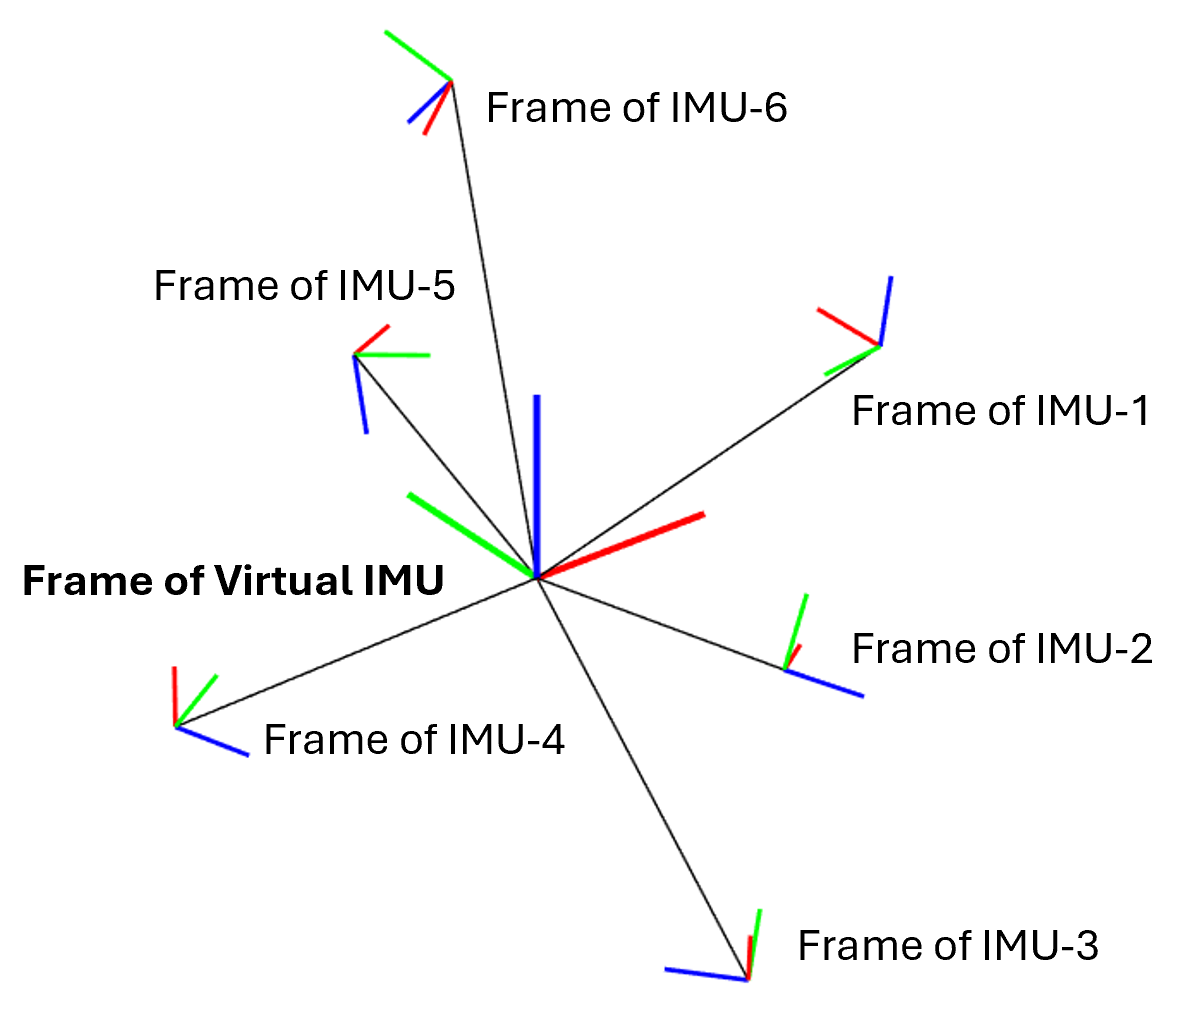
\includegraphics[width=0.7\linewidth]{figures/fig_frame.png}
    % \caption{VIMU frame $\bm{\mathcal{F}}_v$ and individual IMU sensor frame $\bm{\mathcal{F}}_s$}
    \caption{Multiple IMU as one. Virtual IMU from weighted-averaging multiple IMUs}
    \label{fig:vimu_frame}
\end{figure}

\section{Related Work}\label{related_work}

In this section, we will introduce some prior works on fusing multiple IMUs for use in estimation pipeline.

% As summarized in \cite{patel2022_multi-imu} there are mainly three ways of

\subsection{Sensor Level Fusion - Virtual IMU}\label{VIMU}

One approach is to perform fusion of multiple IMUs before using the measurement in inertial navigation system (INS). For example, \cite{jafari2014_PEM} uses Prediction Error Minimization method to model noise of IMUs and uses a Kalman filter to estimate the optimal process signal. \cite{xue2023} proposed to use a Kalman filter to estimate the angular velocity measured by multiple non-orthogonal gyroscopes. Instead of using a Kalman filter, an easier approach would be to directly average multiple gyroscopes after aligned under a common virtual IMU frame as discussed in \cite{waegli2008, patel2022_multi-imu, Colomina2004REDUNDANTIF}.

However, averaging of multiple accelerometers was not considered due to the additional acceleration terms from rotation (lever arm effect), unless they are closely placed and the separations in between are ignored. In section \ref{methodology} we will show how it is possible to average multiple accelerometers even with separations.

\subsection{State Augmentation with Multiple IMUs}\label{augmented}

Typically, a state estimation problem with a IMU involves tracking the orientation, linear velocity, and linear acceleration of the vehicle (commonly defined at the IMU). With additional IMUs, additional state variables such as linear acceleration, angular velocity, and angular acceleration are added. This allows using the full mechanization model of accelerometer as the measurement update in the Kalman filter \cite{Bancroft2011DataFA, Beaudoin2018_satelite}. On the contrary, our approach only involves averaging the measurements thus keeping the computational overhead minimal.

\subsection{Stacked IMU States with Geometric Constraints}\label{constraint}

Another approach is to track the state of each IMU individually and associate them with geometric constraints \cite{waegli2008, Beaudoin2018_satelite}. Using multiple IMUs and cameras, \cite{Eckenhoff2021_MIMC-VINS} proposed to track all stacked states of base and auxillary IMUs using MSCKF \cite{Anastasios2007_MSCKF}. Assuming the extrinsic calibrations of all IMUs are known and fixed, relative geometric constraints are imposed between states of different IMUs in the form of measurement updates in addition to camera observations. Our approach allows fusing the information from multiple IMUs without the need of introducing the extra geometric constraints in the state estimation pipeline.

\subsection{Distributed INS}\label{distributed}

The last common approach is to have an individual state estimator for each IMU system each performing local propagation and correction. Simple state fusion is performed with each estimator's estimate \cite{Bancroft2011DataFA, patel2022_multi-imu}. Our approach avoids the need to run several state estimators which can be expensive.

\subsection{Summary}

As presented, multiple approaches have being proposed. \ref{constraint} would be computationally expensive if the number of IMUs is large as it has many states all in one Kalman filter. The averaging approach in \ref{VIMU} would be the simplest to implement and does not significantly alter the existing single IMU framework. However, due to the lever-arm effect, averaging multiple accelerometers that are physically separated is not visited. We will show that it is still possible to average the accelerometers despite the separation and give a tunable VIMU frame as a result.

\section{Preliminaries}

\subsection{Definitions}

In this discussion, we use the following four frames of references: 1) inertial frame $\bm{\mathcal{F}}_i$, 2) body frame $\bm{\mathcal{F}}_b$ is for expressing sensor extrinsic calibration relative to some mechanical datum, 3) sensor frame $\bm{\mathcal{F}}_s$ is the local frame of reference at each sensor, 4) VIMU frame or Vehicle frame $\bm{\mathcal{F}}_v$ is for tracking vehicle pose in state estimation pipeline.

For any point $\textbf{p}$ or vector we define as $\textbf{r}_i^{pi}$ in the inertial frame $\bm{\mathcal{F}}_i$. For example, the vehicle position in the inertial frame thus becomes $\textbf{r}_i^{vi}$.

When referring to the pose of a vehicle, it is the tuple of $\{\textbf{C}_{iv}, \textbf{r}_i^{vi}\}$, which forms the transformation matrix as follows:
$$
\textbf{T}_{iv} = \left[\begin{matrix}
    \textbf{C}_{iv} & \textbf{r}_i^{vi} \\
    \textbf{0} & 1
\end{matrix}\right].
$$

The pose can be used to transform point $\textbf{r}_v^{pv}$ expressed in vehicle frame $\bm{\mathcal{F}}_v$ into inertial frame $\bm{\mathcal{F}}_i$ as $\textbf{r}_i^{pi}$:
$$
\left[\begin{matrix} \textbf{r}_i^{pi} \\ 1 \end{matrix}\right]
    = \textbf{T}_{iv} \left[\begin{matrix} \textbf{r}_v^{pv} \\ 1 \end{matrix}\right]
\quad \text{or} \quad
\textbf{r}_i^{pi} = \textbf{C}_{iv} \textbf{r}_v^{pv} + \textbf{r}_i^{vi}.
$$

In this document $^\wedge$ is specifically used for rendering an element of $\mathbb{R}^3$ as a skew-symmetric matrix:
$$
\bm{\omega}^\wedge = \left[\begin{matrix}
    0 & -\omega_2 & \omega_1 \\
    \omega_2 & 0 & -\omega_3 \\
    -\omega_1 & \omega_3 & 0
\end{matrix}\right].
$$

If a quantity is in the form $x(t)$, then it is a time-varying quantity, otherwise it is time-invariant.

\subsection{Rigid-Body Kinematics}

The state propagation using IMU measurements follows the rigid-body kinematics in world fixed frame:
\begin{equation}
\begin{split}
    \dot{\textbf{C}}(t) &= \textbf{C}(t) \bm{\omega}(t)^\wedge, \\
    \dot{\textbf{v}}(t) &= \textbf{C}(t) \textbf{a}(t) - \textbf{g}, \\
    \dot{\textbf{p}}(t) &= \textbf{v}(t).
\end{split}
\end{equation}

Here $\textbf{C}$ is short for $\textbf{C}_{iv}$, $\textbf{v}$ is short for $\textbf{v}_i^{vi}$, and $\textbf{p}$ is for the position of the vehicle $\textbf{r}_i^{vi}$. These three form a 9-DOF state.

In addition, $\textbf{g}$ is the acceleration from gravity and $\bm{\omega}$ and $\textbf{a}$ are the true angular velocity and true linear acceleration in the vehicle frame.

\subsection{IMU Measurement Model}

For the angular velocity measurement from a gyroscope we have the following measurement model:

\begin{equation}
    \textbf{y}_\omega(t) = \bm{\omega}(t) + \textbf{b}_\omega(t) + \textbf{n}_\omega(t),
\end{equation}

\noindent where $\textbf{b}_\omega$ is the bias of gyroscope measurement due to random walk and $\textbf{n}_\omega$ is the additive white noise of the measurement. Similarly, we have the following measurement model for an accelerometer at the vehicle frame:

\begin{equation}
    \textbf{y}_a(t) = \textbf{a}(t) + \textbf{b}_a(t) + \textbf{n}_a(t),
\end{equation}

\noindent here $\textbf{b}_a$ is the bias of accelerometer and $\textbf{n}_a$ is the noise of the acceleration measurement.

Bias drifts of IMU are modeled as random walk with the bias drift rate sampled from a Gaussian noise:
\begin{equation}
\begin{split}
    \dot{\textbf{b}}_\omega(t) &= \textbf{w}_\omega(t), \\
    \dot{\textbf{b}}_a(t) &= \textbf{w}_a(t).
\end{split}
\end{equation}

\noindent Due to the presence of biases, it is estimated as part of the state vector and subtracted from the raw measurement to get the "unbiased" measurement for propagation:
\begin{equation}
\begin{split}
    \hat{\bm{\omega}}(t) = \textbf{y}_\omega(t) - \hat{\textbf{b}}_\omega(t), \\
    \hat{\textbf{a}}(t)  = \textbf{y}_a(t) - \hat{\textbf{b}}_a(t).
\end{split}
\end{equation}

For an IMU not located at the vehicle frame, measurements are in each IMU's local frame and we have additional terms in the acceleration measurement due to lever arm effect:
\begin{equation}
\begin{split}
    \textbf{y}_{\omega,i}(t) &= \textbf{C}_{i}^{-1} \bm{\omega}(t) + \textbf{b}_{\omega, i}(t) + \textbf{n}_{\omega,i}(t), \\
    \textbf{y}_{a,i}(t) &= \textbf{C}_i^{-1} \left[ \textbf{a}(t) + \bm{\omega}(t)^\wedge (\bm{\omega}(t)^\wedge \textbf{r}_i) + \bm{\alpha}(t)^\wedge \textbf{r}_i \right] \\
    &+ \textbf{b}_{a,i}(t) + \textbf{n}_{a,i}(t).
\end{split}
\end{equation}

\noindent Here we have $\textbf{C}_i$ and $\textbf{r}_i$ short for $\textbf{C}_{vs}$ and $\textbf{r}_v^{sv}$ defining the pose $\textbf{T}_{vs}$ of the $i$-th IMU in the vehicle frame.

\section{Methodology}\label{methodology}

\subsection{Averaging Multiple Gyroscopes}

First, we align the gyroscope measurements with the vehicle frame:
\begin{equation}
    \textbf{C}_{i} \textbf{y}_{\omega,i}(t) = \bm{\omega}(t) + \textbf{C}_{i} \textbf{b}_{\omega, i}(t) + \textbf{C}_{i} \textbf{n}_{\omega,i}(t).
\end{equation}

\noindent The weighted average of all gyroscopes is simply,
\begin{equation}
\begin{split}
    \bar{\textbf{y}}_\omega(t) &= \sum_i{w_i \textbf{C}_{i} \textbf{y}_{\omega,i}(t)} \\
    &= \sum_i{w_i \left( \bm{\omega}(t) + \textbf{C}_{i} \textbf{b}_{\omega,i}(t) + \textbf{C}_{i} \textbf{n}_{\omega,i}(t) \right)} \\
    &= \bm{\omega}(t) + \sum_i{w_i \textbf{C}_{i} \textbf{b}_{\omega,i}(t)} + \sum_i{w_i \textbf{C}_{i} \textbf{n}_{\omega,i}(t)}
\end{split}
\end{equation}

\noindent Where $w_i$ are the weights with $\sum_i{w_i} = 1$.

We see that the averaged measurement can be summarized as
\begin{equation}
    \bar{\textbf{y}}_\omega(t) = \bm{\omega}(t) + \bar{\textbf{b}}_\omega(t) + \bar{\textbf{n}}_\omega(t),
\end{equation}

\noindent where $\bar{\textbf{b}}_\omega(t) = \sum_i{w_i \textbf{C}_{i} \textbf{b}_{\omega,i}(t)}$ and $\bar{\textbf{n}}_\omega(t) = \sum_i{w_i \textbf{C}_{i} \textbf{n}_{\omega,i}(t)}$ are the combined biases and noises.

\subsection{Averaging Multiple Accelerometers}

Aligning all accelerometer measurements to the vehicle frame, we have
\begin{equation}\label{eqn_accel}
\begin{split}
    \textbf{C}_{i} \textbf{y}_{a,i}(t) &= \textbf{a}(t) + \bm{\omega}(t)^\wedge (\bm{\omega}(t)^\wedge \textbf{r}_i) + \bm{\alpha}(t)^\wedge \textbf{r}_i \\
    &+ \textbf{C}_{i} \textbf{b}_{a,i}(t) + \textbf{C}_{i} \textbf{n}_{a,i}(t)
\end{split}
\end{equation}

\noindent Summing (\ref{eqn_accel}) over all accelerometers gives
\begin{equation}
\begin{split}
    \bar{\textbf{y}}_a(t) &= \sum_i{w_i \textbf{C}_{i} \textbf{y}_{a,i}(t)} \\
    &= \textbf{a}(t) + \sum_i{w_i \textbf{C}_{i} \textbf{b}_{a,i}(t)} + \sum_i{w_i \textbf{C}_{i} \textbf{n}_{a,i}(t)} \\
    &+ \sum_i{w_i \bm{\omega}(t)^\wedge (\bm{\omega}(t)^\wedge \textbf{r}_i)} + \sum_i{w_i \bm{\alpha}(t)^\wedge \textbf{r}_i} \\
\end{split}
\end{equation}

\noindent Using the fact that $^\wedge$ is linear, we have
\begin{equation}\label{accel_avg_final}
\begin{split}
    \bar{\textbf{y}}_a(t) &= \sum_i{w_i \textbf{C}_{i} \textbf{y}_{a,i}(t)} \\
    &= \textbf{a}(t) + \sum_i{w_i \textbf{C}_{i} \textbf{b}_{a,i}(t)} + \sum_i{w_i \textbf{C}_{i} \textbf{n}_{a,i}(t)} \\
    &+ \bm{\omega}(t)^\wedge \left(\bm{\omega}(t)^\wedge \left( \sum_i{w_i \textbf{r}_i} \right) \right) + \bm{\alpha}(t)^\wedge \left( \sum_i{w_i\textbf{r}_i} \right).
\end{split}
\end{equation}

\noindent We see that if $\sum_i{w_i \textbf{r}_i} = \textbf{0}$, then we can {\em eliminate} the last two terms from the lever-arm effect. This simplifies (\ref{accel_avg_final}) to
\begin{equation}
    \bar{\textbf{y}}_a(t) = \textbf{a}(t) + \bar{\textbf{b}}_a(t) + \bar{\textbf{n}}_a(t).
\end{equation}

\subsection{VIMU from Weighted Average}\label{AA}

As we can see, if we choose the vehicle frame and weights of theaccelerometers such that $\sum_i{w_i \textbf{r}_i} = \textbf{0}$, then we can ignore the separation of all IMUs and fuse the accelerometer measurements through averaging. The result is an virtual IMU at the weighted centroid without any lever-arm effects.

Since gyroscope measurement is location independent, we can choose different weights for averaging gyroscopes and accelerometers.

Because all biases are slowly varying, the combined biases are also slowly varying. Therefore, instead of tracking individual biases, only the combined biases are needed. When receiving a new set of IMU measurements, we estimate the angular velocity and linear acceleration with the simple update equations below:
\begin{equation}
\begin{split}
    \hat{\bm{\omega}}(t) = \bar{\textbf{y}}_\omega(t) - \hat{\bar{\textbf{b}}}_\omega(t), \\
    \hat{\textbf{a}}(t)  = \bar{\textbf{y}}_a(t) - \hat{\bar{\textbf{b}}}_a(t).
\end{split}
\end{equation}

The combined measurements are expected to have slower drift and the estimate is expected to be less noisy as well \cite{patel2022_multi-imu}. If having $n$ identical IMUs and equal weights the standard deviation of the combined noise or drift rate is expected to be $\bar{\sigma} = \sigma / \sqrt{n}$.
% \begin{equation}
%     \bar{\sigma} = \frac{\sigma}{\sqrt{n}}
% \end{equation}

\subsection{Selecting Weights for Minimal Uncertainty}\label{solve_weight_by_noise}

When selecting weights for gyroscopes, or for accelerometers under the condition that the selection of vehicle frame is flexible, we can minimize the output noise or bias drift rate. Below, we take the bias drift as an example but similar ideas can be applied to the output noise.

The combined drift rate is as follows.
\begin{equation}
    \dot{\bar{\textbf{b}}}(t) = \sum_i{w_i \textbf{C}_i \textbf{w}_i(t)}.
\end{equation}

\noindent Here we drop the subscript as it is the same for both gyroscope drift and accelerometer drift. The covariance of the combined drift rate is the weighted sum of the noise covariances of each IMU:
\begin{equation}
    \bar{\bm{\Sigma}} = \sum_i{w_i^2 \bm{\Sigma}_i}.
\end{equation}

\noindent We can then solve for the weights that minimize the trace of the combined covariance.

If the IMU have isotropic noise for all three axes, the combined variance simplifies to
\begin{equation}\label{noise_reduction_asym}
    \bar{\sigma}^2 = \sum_i{w_i^2 \sigma_i^2}.
\end{equation}

\noindent Furthermore, if using $n$ of the same IMUs and equal weighting, the combined variance is simply
\begin{equation}\label{noise_reduction_sym}
    \bar{\sigma}^2 = \sum_i{w_i^2 \sigma^2} = n \left(\frac{\sigma}{n}\right)^2 = \frac{\sigma^2}{n}.
\end{equation}

\subsection{Selecting Weights for VIMU Frame Placement}

Given that $\sum_i{w_i \textbf{r}_i} = \textbf{0}$, if there are only two IMUs, we can only place the VIMU frame on the line through the center of the two IMUs. If there are three IMUs, we can only place the VIMU frame on the plane formed by the three IMUs. If there are four non-coplanar IMUs, then in theory, we can place the VIMU frame anywhere. However, placing the VIMU frame outside of the convex hull of the IMUs will increase the output noise which is usually not desirable.

When we have a target vehicle frame in mind, we need to solve for the required weights. Assuming we have arbitrarily many IMUs, then the problem can be formulated as an optimization problem:
\begin{equation}\label{opt_problem}
\begin{split}
    \min_{w_i}{\frac{1}{2} \sum{w_i^2 \sigma_i^2}} \quad \text{s.t. }
    \begin{cases}
      \sum_i{w_i \textbf{r}_i} &= \textbf{0} \\
      \sum_i{w_i} &= 1
    \end{cases}
\end{split}
\end{equation}

\noindent Here $\textbf{r}_i$ is the relative position of the IMUs to the selected VIMU frame. We chose the objective to reduce output noise as shown in section \ref{solve_weight_by_noise}. Since (\ref{opt_problem}) is a quadratic programming problem, it is possible to find a closed-form solution.

The Lagrangian of the problem is $\mathcal{L} = \frac{1}{2}\textbf{w}^T \bm{\Sigma} \textbf{w} + \bm{\lambda}^T \textbf{R}\textbf{w} + \beta \left( 1 - \textbf{1}^T \textbf{w} \right)$ where $\textbf{w}^T = \left[\begin{matrix} w_1 \dots w_n \end{matrix}\right]$, $\bm{\Sigma} = \text{diag}(\sigma_1^2, ..., \sigma_n^2)$, $\textbf{R} = \left[\begin{matrix} \textbf{r}_0 \dots \textbf{r}_n\end{matrix}\right]$ and $\textbf{1}^T = \left[\begin{matrix}1 \dots 1\end{matrix}\right]$. This gives the following KKT conditions:
\begin{equation}
\begin{split}
  \bm{\Sigma}\textbf{w} + \textbf{R}^T \bm{\lambda} - \beta \textbf{1} &= \textbf{0} \\
  \textbf{R} \textbf{w} &= \textbf{0} \\
  \textbf{1}^T \textbf{w} &= 1
\end{split}
\end{equation}

\noindent If we left multiple the first KKT condition by $\textbf{w}^T$, we have
\begin{equation}
\textbf{w}^T\bm{\Sigma}\textbf{w} + \textbf{w}^T\textbf{R}\bm{\lambda} - \beta \textbf{w}^T\textbf{1} = 0.
\end{equation}

\noindent Since $\textbf{w}^T\textbf{R} = \textbf{0}$ and $\textbf{1}\textbf{w} = 1$ this implies
\begin{equation}\label{beta}
    \beta = \textbf{w}^T\bm{\Sigma}\textbf{w}.
\end{equation}

\noindent Left multiplying the first KKT condition by $\bar{\textbf{R}} = \textbf{R}\bm{\Sigma}^{-1}$ gives
\begin{equation}
\underbrace{\textbf{R}\textbf{w}}_{=\textbf{0}} + \bar{\textbf{R}}\textbf{R}^T\bm{\lambda} - \beta\bar{\textbf{R}}\textbf{1} = 0.
\end{equation}

\noindent Here we define $\bar{\textbf{r}} = \bar{\textbf{R}}\textbf{1} = \sum{\textbf{r}_i / \sigma_i^2}$ and using the pseudo-inverse of $\bar{\textbf{R}}\textbf{R}^T$, we have

% assuming $\textbf{R}\textbf{R}^T$ is invertible due to having at least 3 non-colocated IMUs then we have,
\begin{equation}\label{lambda}
    \bm{\lambda} = \beta \left(\bar{\textbf{R}}\textbf{R}^T\right)^{+} \textbf{r}.
\end{equation}

\noindent Substitute equations (\ref{beta}) and (\ref{lambda}) into first KKT condition we have,
\begin{equation}
    \hat{\textbf{w}} = \frac{\textbf{w}}{\textbf{w}^T\bm{\Sigma}\textbf{w}} = \bm{\Sigma}^{-1} \left( \textbf{1} - \textbf{R}^T \left(\bar{\textbf{R}}\textbf{R}^T\right)^{+} \bar{\textbf{r}} \right).
\end{equation}

\noindent Lastly, since $\sum_i{w_i} = 1$, we need to normalize the intermediate solution to get the final weights for the accelerometers:
\begin{equation}
    \textbf{w}^* = \frac{\hat{\textbf{w}}}{\textbf{1}^T \hat{\textbf{w}}}.
\end{equation}

\section{Simulation} \label{simulation}

To check the correctness of the frame-selection method through weighted averaging, and to show performance benefit of the fused VIMU, we first performed evaluation in simulation.

\subsection{Data Generation}

To generate the simulated data, we used different combination of sinusoidal functions to generate the ground truth angular velocity and linear acceleration in the body frame as shown in Figure \ref{fig:omega} and Figure \ref{fig:accel}. Then we integrate them to generate the ground-truth trajectory. We selected MPU6050, a common MEMS IMU in the mechatronics community as the example model. For each IMU, we simulate its measurements given the relative transformation in the body frame and added noises and biases. Each IMU is sampled at 100 Hz. These are done using utilities \texttt{kinematicTrajectory} and \texttt{imuSensor} provided by MATLAB.

% \begin{figure}[t!]
%     \centering
%     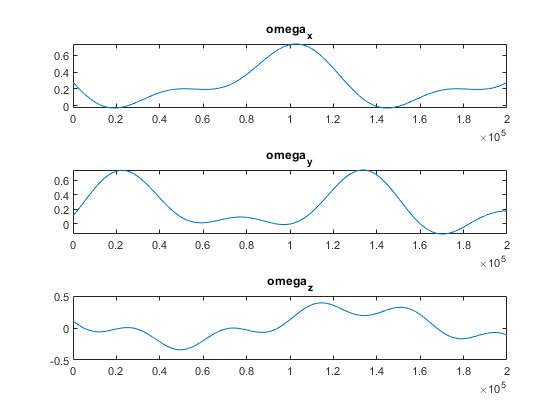
\includegraphics[width=1.0\linewidth]{figures/simulated_omega.png}
%     \caption{Simulated Angular Velocity}
%     \label{fig:omega}
% \end{figure}

% \begin{figure}[t!]
%     \centering
%     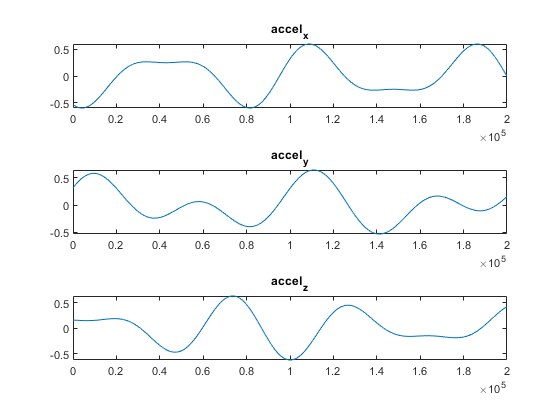
\includegraphics[width=1.0\linewidth]{figures/simulated_accel.png}
%     \caption{Simulated Linear Acceleration}
%     \label{fig:accel}
% \end{figure}

\begin{figure*}[ht]
    \centering
    \begin{subfigure}[b]{0.45\linewidth}
        \centering
        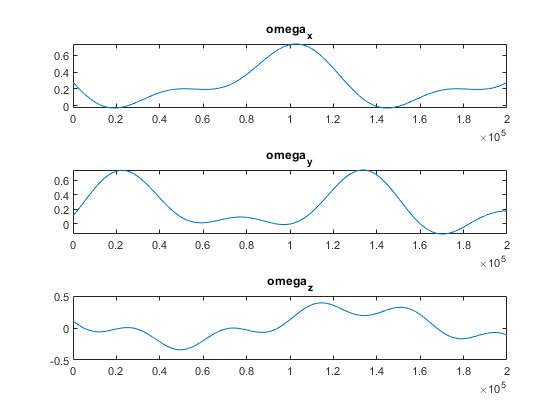
\includegraphics[width=9cm]{figures/simulated_omega.png}
        \caption{Simulated Angular Velocity}
        \label{fig:omega}
    \end{subfigure}
    \begin{subfigure}[b]{0.45\linewidth}
        \centering
        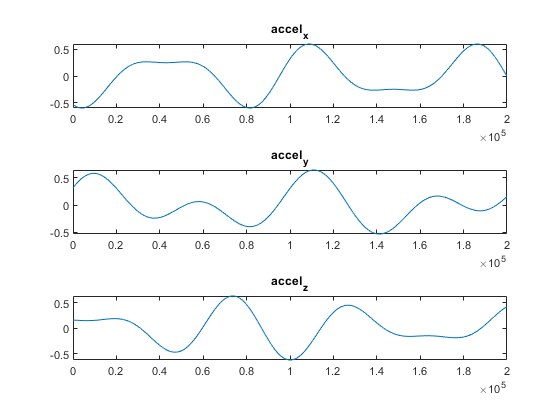
\includegraphics[width=9cm]{figures/simulated_accel.png}
        \caption{Simulated Linear Acceleration}
        \label{fig:accel}
    \end{subfigure}
\caption{Simulated kinematics for ground-truth trajectory generation}
\label{fig:simulation_data}
\end{figure*}

\subsection{Implementation}

We also simulate observations of known landmarks from a monocular camera at body frame. This turns the estimation problem into a localization problem such that the error is bounded. For each camera frame, we first sample random observations in the imaging plane as well as depth (between 2 and 10 m). We perform reprojection and transform the resulted 3D points to the inertial frame with the ground-truth pose to generate the corresponding landmark positions. Camera observations arrive at 2 Hz. We selected this low update rate to allow error to propagate for better showing the benefits of averaging.

For the estimator, we implemented the \textit{left-}Invariant Extended Kalman Filter (IEKF) \cite{IEKF} as it is more accurate compared to standard EKF methods. At initialization stage, given all IMU poses, we compute the weighting that places the VIMU frame at the body frame, which is also the camera frame. Using the weights, we also calculate the combined noises and bias drift rates. When new IMU measurements arrive, they are weighted averaged and then fed into the estimator as though we have a single IMU. When camera observations arrive, the 2D observations and 3D landmark positions are used for the correction step.

\subsection{Experiment Setup}

For performance, we compared results of multiple different IMU configurations summarized in Table \ref{tab:imu_config}. Here symmetric configurations have IMUs placed along the principal axes with an offset of 1 m with random orientation. Assymmetric configurations use IMUs perturbed from the symmetric configuration such that unequal weightings are required to have VIMU frame at origin of body frame. We place the VIMU frame at the body frame for all configurations to give a fair comparison of performance (direct comparison with ground truth). Poses of all IMUs used are plotted in Figure \ref{fig:imu_configurations}.

\begin{table}[h!]
\centering
\caption{Different IMU Configurations}
\label{tab:imu_config}
\begin{tabular}{cccc}
\toprule
\textbf{Configuration} & \textbf{Category} & \textbf{\# of IMUs} & \textbf{IMU used}  \\
\midrule
IMU-S0 & Baseline  & 1 & 0 \\
\midrule
IMU-S2 & Symmetric & 2 & 1, 2 \\
IMU-S4 & Symmetric & 4 & 1, 2, 3, 4 \\
IMU-S6 & Symmetric & 6 & 1, 2, 3, 4, 5, 6 \\
\midrule
IMU-A2 & Asymmetric & 2 & 11, 12 \\
IMU-A4 & Asymmetric & 4 & 11, 12, 13, 14 \\
IMU-S6 & Asymmetric & 6 & 11, 12, 13, 14, 15, 16 \\

\bottomrule
\end{tabular}
\end{table}

% \begin{table}[h!]
% \centering
% \caption{Pose of IMUs}
% \label{tab:imu_pose}
% \begin{tabular}{ccc}
% \toprule
% \textbf{IMU ID} & \textbf{orientation} & \textbf{position} \\
% \midrule
% 0      & $1.000 +0.000i +0.000j + 0.000k$ & [$+0.0, +0.0, +0.0$] \\
% \midrule
% 1      & $0.633 +0.065i -0.025j +0.771k$ & [$+1.0, +0.0, +0.0$] \\
% 2      & $0.395 +0.795i +0.322j +0.328k$ & [$-1.0, +0.0, +0.0$] \\
% 3      & $0.533 -0.314i +0.671j +0.409k$ & [$+0.0, +1.0, +0.0$] \\
% 4      & $0.600 +0.323i +0.620j +0.390k$ & [$+0.0, -1.0, +0.0$] \\
% 5      & $0.231 +0.495i +0.343j -0.764k$ & [$+0.0, +0.0, +1.0$] \\
% 6      & $0.744 -0.473i +0.355j +0.310k$ & [$+0.0, +0.0, -1.0$] \\
% \midrule
% 11     & $0.045 -0.112i +0.670j +0.733k$ & [$+0.9, +0.0, +0.0$] \\
% 12     & $0.223 -0.059i +0.929j -0.289k$ & [$-1.2, +0.0, +0.0$] \\
% 13     & $0.119 +0.962i +0.245j -0.031k$ & [$+0.3, +1.1, +0.0$] \\
% 14     & $0.605 +0.708i +0.335j +0.141k$ & [$+0.2, -0.7, +0.0$] \\
% 15     & $0.004 -0.299i +0.894j +0.333k$ & [$-0.1, +0.2, +1.3$] \\
% 16     & $0.598 -0.094i -0.669j -0.432k$ & [$+0.4, -0.3, -1.1$] \\
% \bottomrule
% \end{tabular}
% \end{table}

% \begin{figure}
%     \centering
%     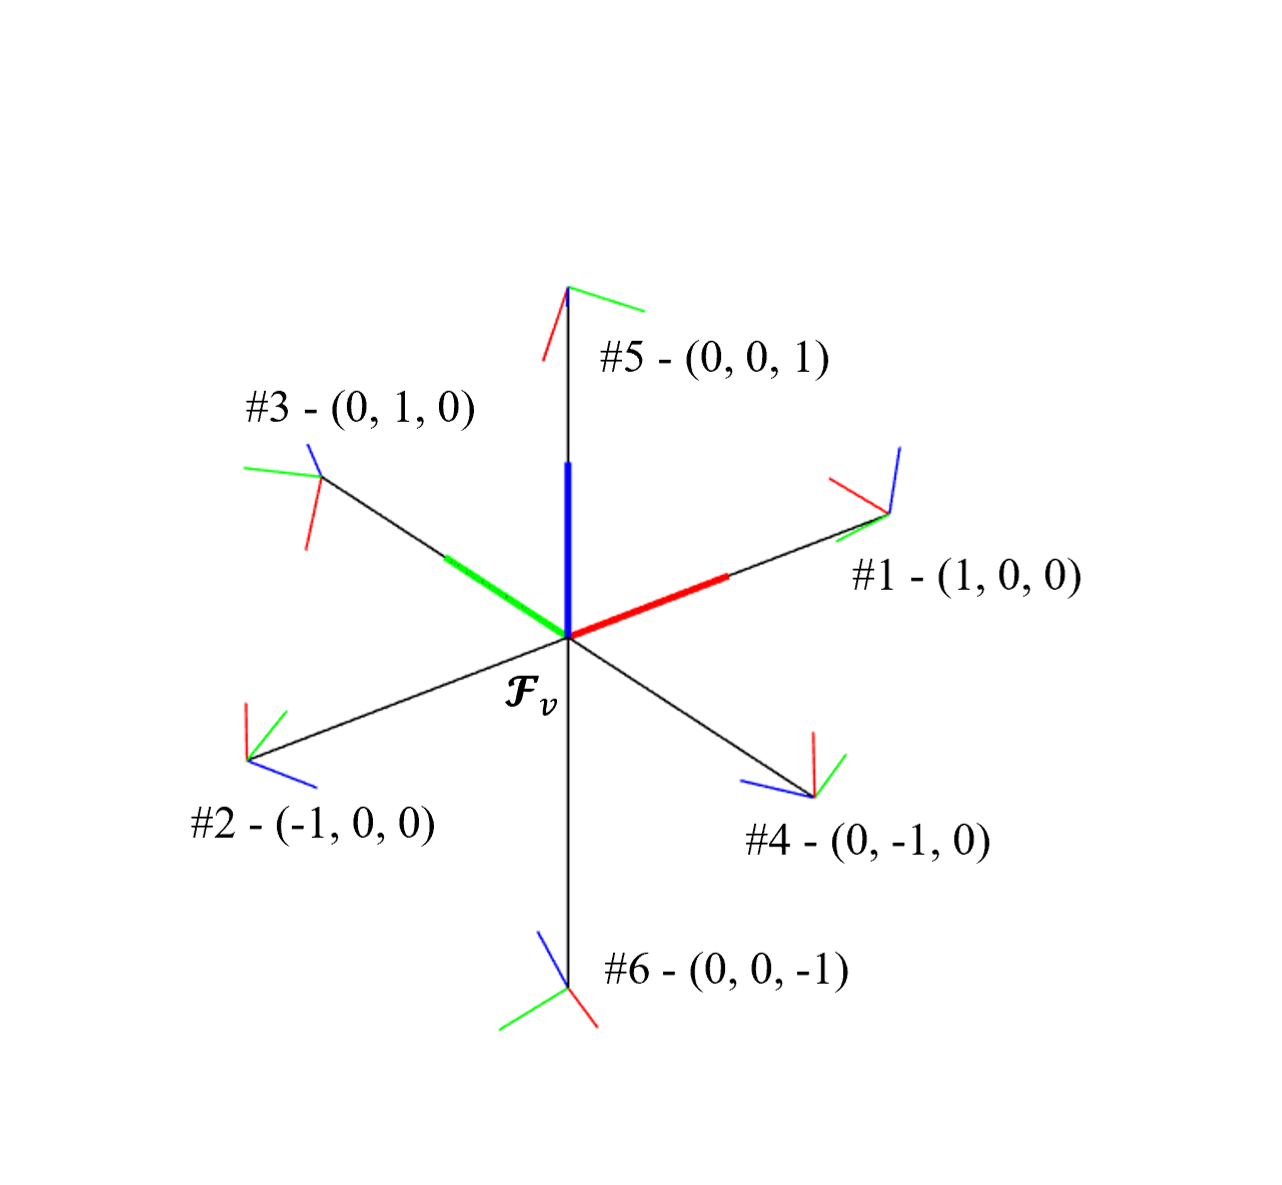
\includegraphics[width=0.75\linewidth]{figures/fig_sym_cropped.png}
%     \caption{Caption}
%     \label{fig:enter-label}
% \end{figure}

% \begin{figure}
%     \centering
%     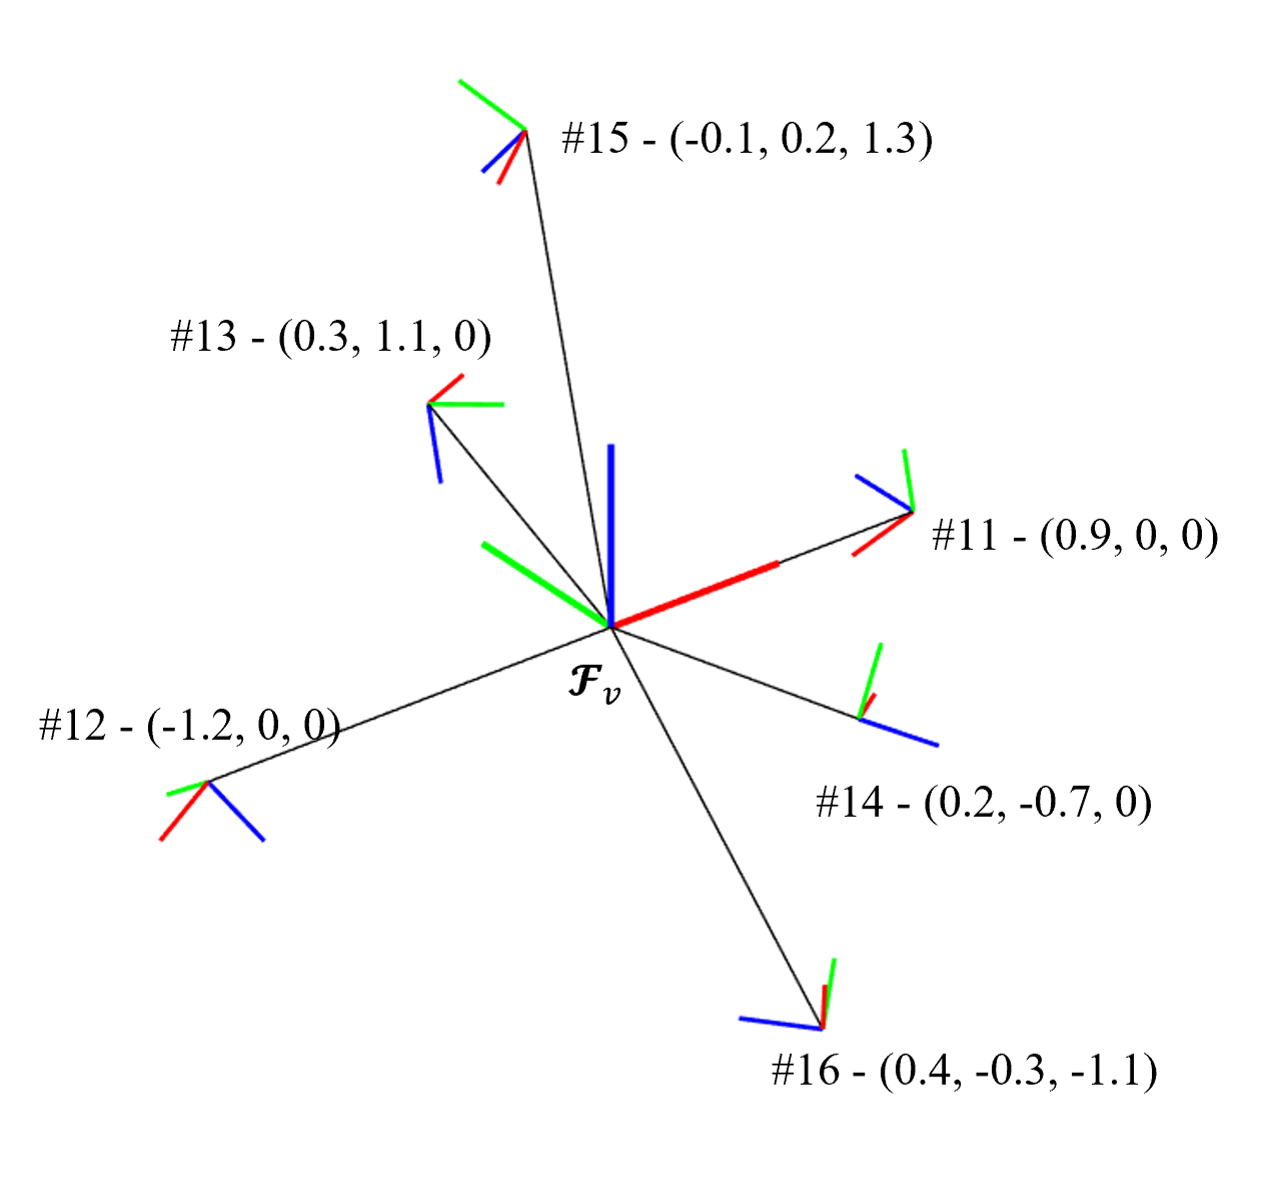
\includegraphics[width=0.75\linewidth]{figures/fig_asym_cropped.png}
%     \caption{Caption}
%     \label{fig:enter-label}
% \end{figure}

\begin{figure*}[ht]
    \centering
    \begin{subfigure}[b]{0.45\linewidth}
        \centering
        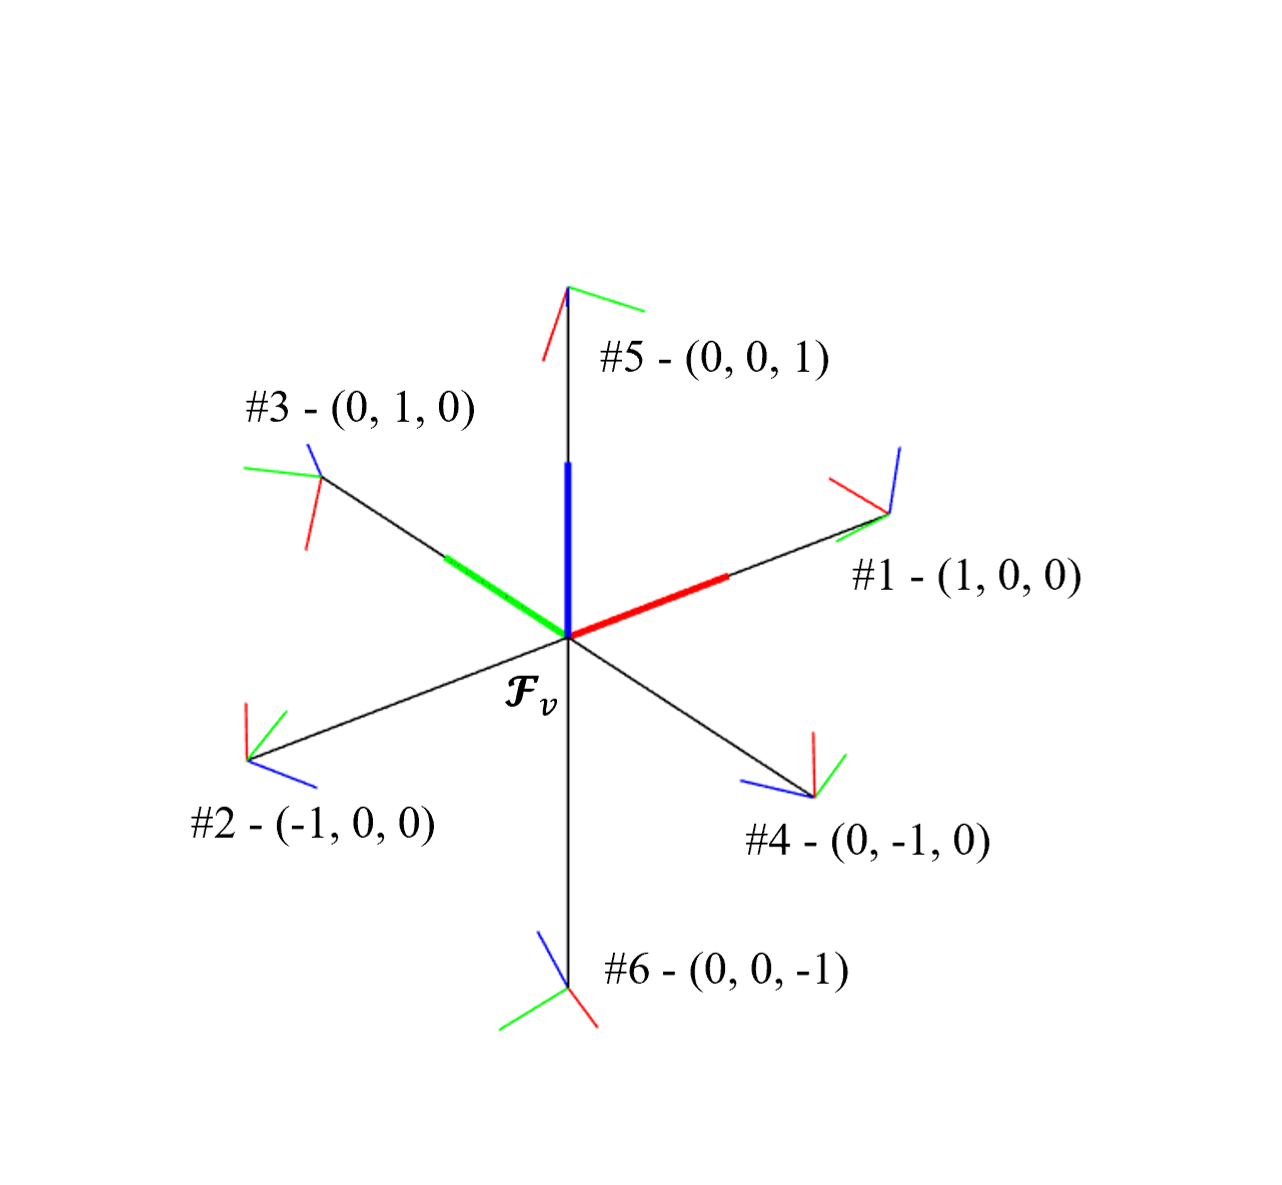
\includegraphics[width=6cm]{figures/fig_sym_cropped.png}
        \caption{Symmetrical IMU placement}
        \label{fig:sym_imu}
    \end{subfigure}
    \begin{subfigure}[b]{0.45\linewidth}
        \centering
        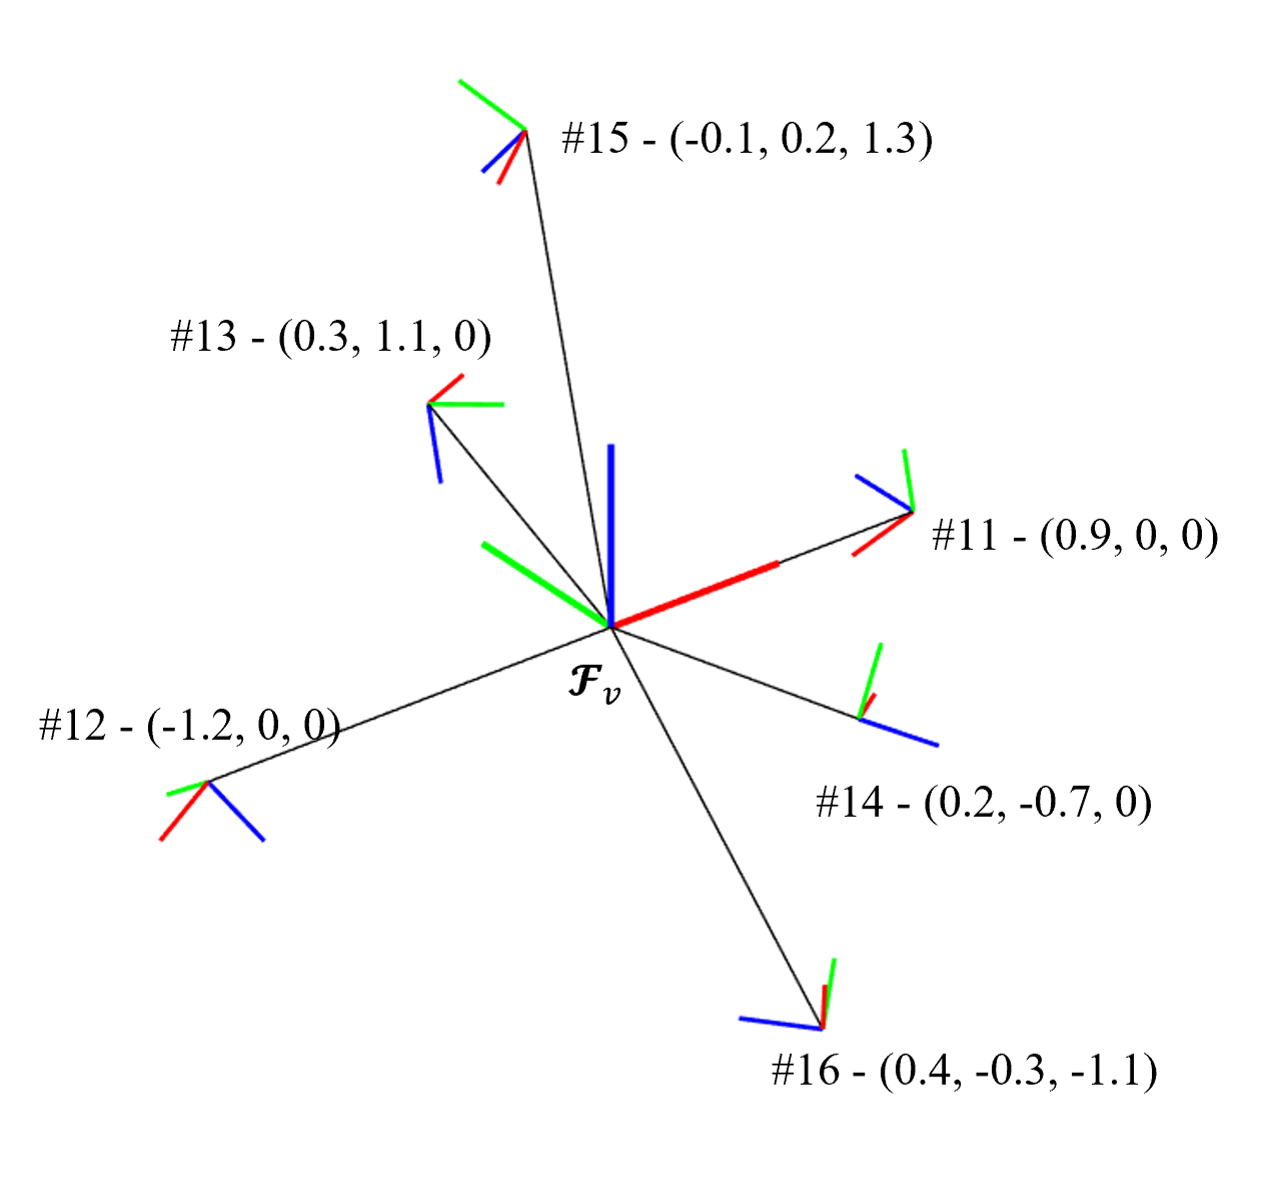
\includegraphics[width=6cm]{figures/fig_asym_cropped.png}
        \caption{Asymmetric IMU placement}
        \label{fig:_asym_imu}
    \end{subfigure}
\caption{Poses of IMUs in different configurations }
\label{fig:imu_configurations}
\end{figure*}

\subsection{Results}

The results are summarized in Table \ref{tab:sim_result}. As more and more IMUs are fused, the mean errors decrease. This matches with the expectation as the combined noises from fused IMU are attenuated as shown by (\ref{noise_reduction_asym}) and (\ref{noise_reduction_sym}). Comparing asymmetric configurations against symmetric configurations, the errors are marginally larger. This can be explained by the unequal weighting, which gives higher level of noises than equal weighting given that all IMUs are identical. Overall, the results suggest averaging between IMUs works for both gyroscope and accelerometer measurements. The combined measurements are also more accurate.

\begin{table}[h!]
\centering
\caption{Simulation Results}
\label{tab:sim_result}
\begin{tabular}{ccccccc}
\toprule
\textbf{Configuration} & \multicolumn{2}{c}{\textbf{Attitude Err (rad)}} & \multicolumn{2}{c}{\textbf{Position Err (m)}} \\
\cmidrule(lr){2-3} \cmidrule(lr){4-5}
& MAE & RMSE & MAE & RMSE \\
\midrule
IMU-S0 & 0.01568 & 0.01873 & 0.11189 & 0.13260 \\
\midrule
IMU-S2 & 0.01278 & 0.01486 & 0.10029 & 0.11540 \\
IMU-S4 & 0.01122 & 0.01319 & 0.09223 & 0.10598 \\
IMU-S6 & 0.01028 & 0.01176 & 0.08950  & 0.10271 \\
\midrule
IMU-A2 & 0.01306 & 0.01514 & 0.10055 & 0.11685 \\
IMU-A4 & 0.01129 & 0.01285 & 0.09222 & 0.10554 \\
IMU-A6 & 0.01083 & 0.01221 & 0.08944 & 0.10077 \\
\bottomrule
\end{tabular}
\end{table}

\section{Real-World Experiment}\label{real_experiment}

For real-world experiments, we chose to perform visual-inertial odometry to understand the performance of averaging in a realistic scenario.

\subsection{Dataset}

Most public datasets only contain a single IMU. We found that the PennCOSYVIO dataset \cite{penncosyvio} meets our needs of containing data from multiple IMUs. This dataset contains 4 different runs with sensor data from three IMUs and multiple cameras as shown in Figure \ref{fig:sensor_on_rig}. For our experiment, we chose to only use the VI sensor camera as it was provided with complete information regarding intrinsic, extrinsic, and distortion information. We also only used the left camera of the VI sensor such that it forms the minimal configuration with a single IMU. This is to better expose the impact of IMUs on performance. We select the VI sensor IMU as the main IMU as it is more accurate compared to the IMUs in the two Tango devices. We will be comparing the performance of using only the VI sensor IMU vs. VIMU from averaging all three IMUs.

\subsection{Implementation}

For VIO implementation, we selected OpenVINS \cite{openvins} to test the different IMU configurations. OpenVINS is based on the MSCKF and supports a single IMU with multiple cameras. It can also estimate cameras and IMU intrinsics as well as time offset and extrinsics between IMU and cameras. After some tuning, we found that enabling extrinsic and time offset estimation gives the best result over many repeated runs. Also since the PennCOSYVIO dataset doesn't have the initialization phase when the vehicle is at rest, we enable dynamic initialization in OpenVINS to estimate initial velocity and biases in motion.

\begin{figure}[h]
\centering
\begin{subfigure}{0.35\textwidth}
\centering
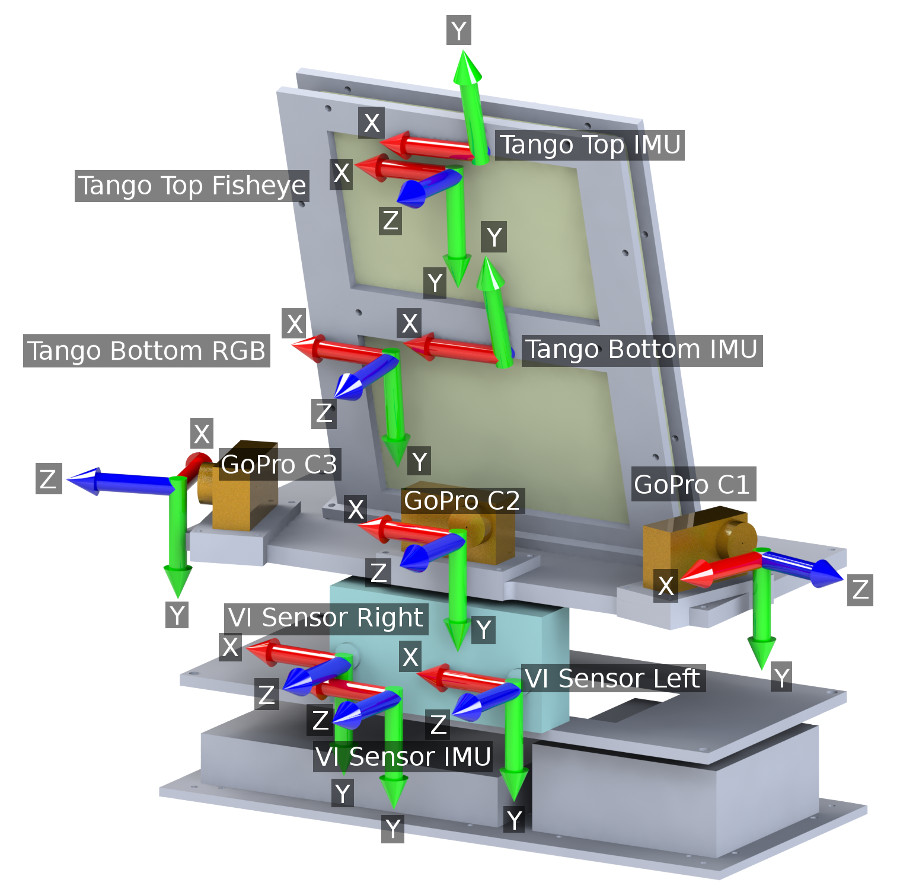
\includegraphics[width = \textwidth]{figures/rig.jpg}
\caption{Sensors}
\label{fig:sensor_on_rig}
\end{subfigure}
\begin{subfigure}{0.12\textwidth}
\centering
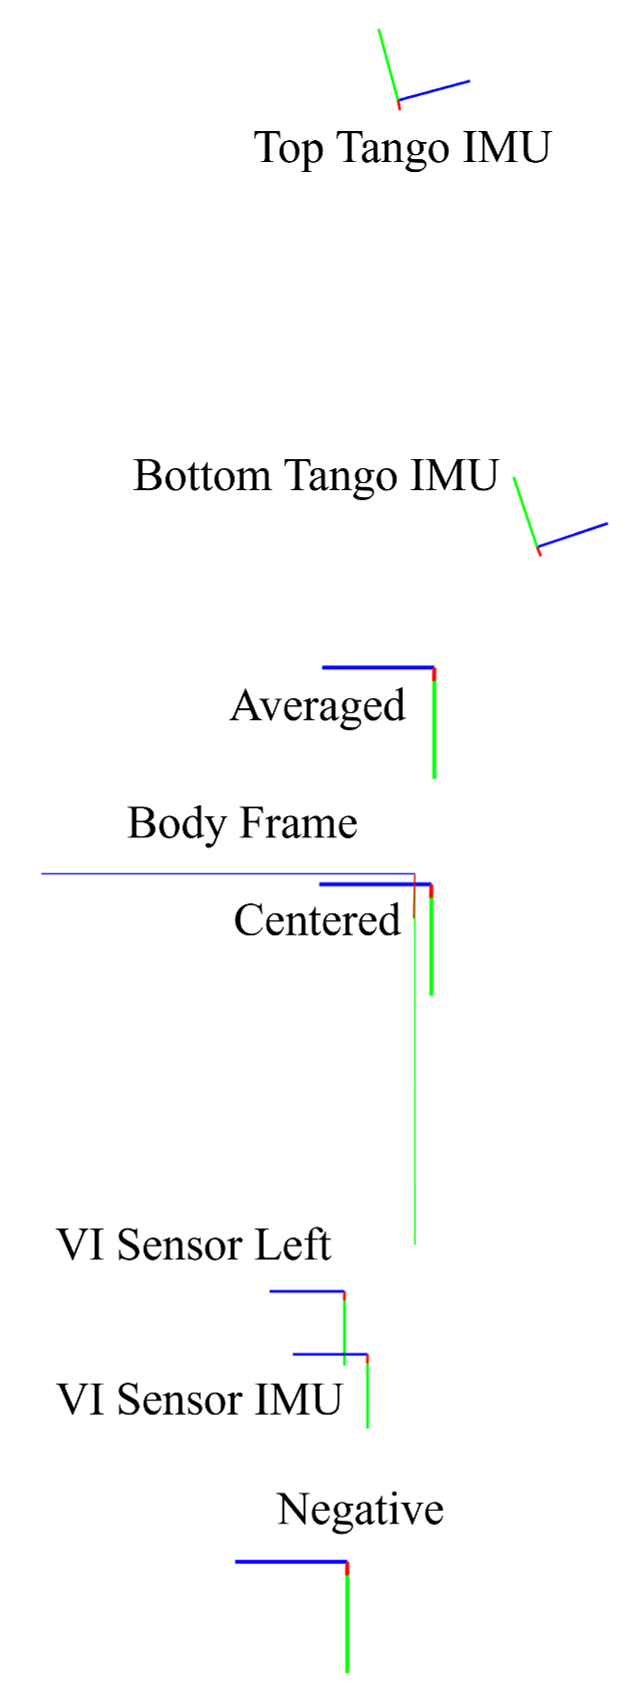
\includegraphics[width = \textwidth]{figures/rig_cropped.png}
\caption{Ref. Frames}
\label{fig:rig_coordinate_frame}
\end{subfigure}
\caption{(a) shows the type and location of sensors on the test rig. (b) shows the various frame of reference used in the experiments viewing from the side}
\label{fig:combined}
\end{figure}

% \begin{figure}
%     \centering
%     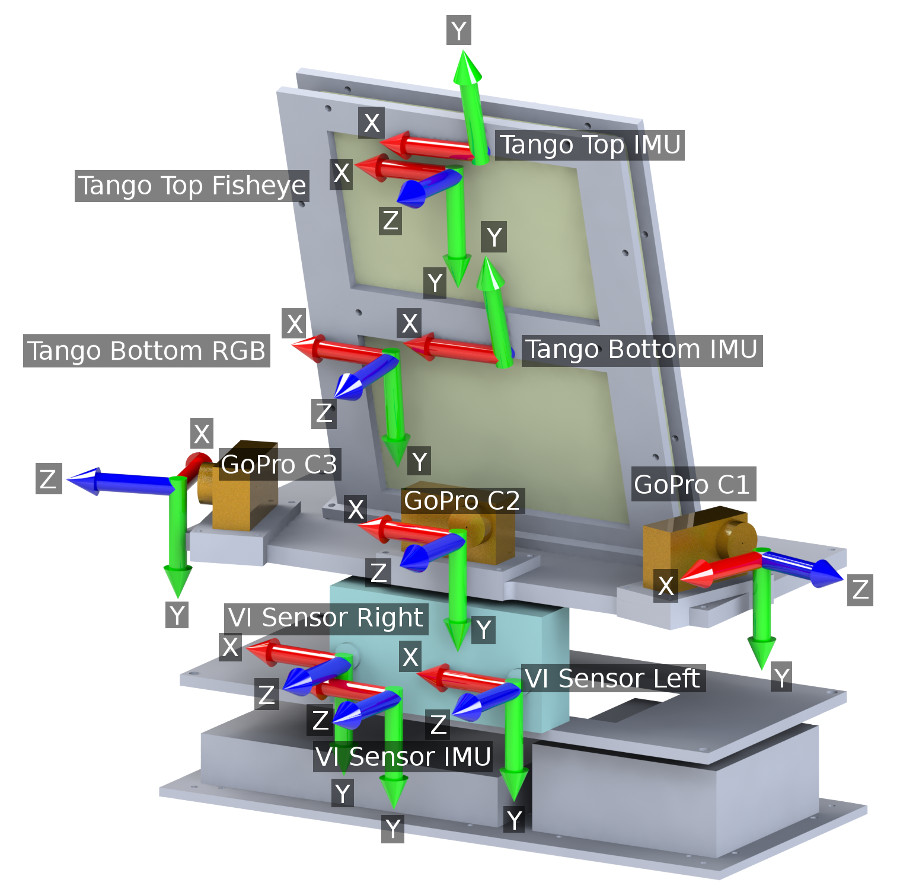
\includegraphics[width=0.75\linewidth]{figures/rig.jpg}
%     \caption{Caption}
%     \label{fig:enter-label}
% \end{figure}

% \begin{figure}
%     \centering
%     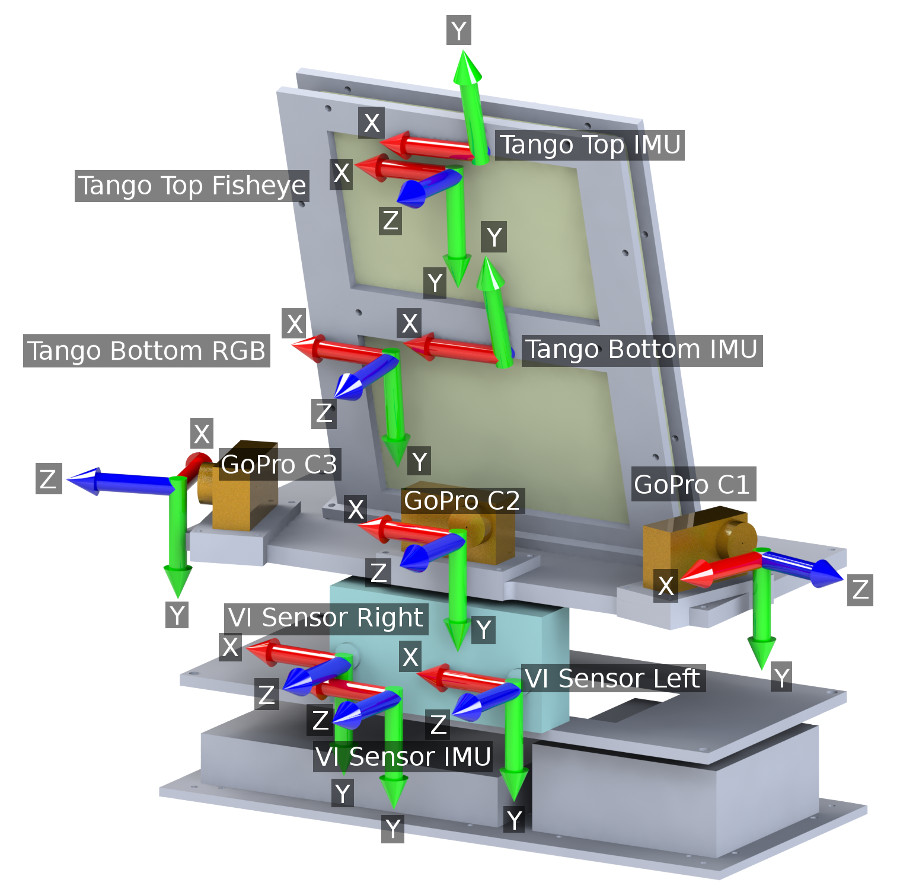
\includegraphics[width=0.75\linewidth]{figures/rig.png}
%     \caption{Caption}
%     \label{fig:enter-label}
% \end{figure}

\subsection{Setup}

To demonstrate that the weighting works as expected, we designed four configurations to test: 1) single IMU with weights $[\begin{matrix} 1.0 & 0.0 & 0.0 \end{matrix}]$ (here the first weight is for VI sensor IMU, second weight for top Tango IMU, and the third weight is for bottom Tango IMU), 2) averaged VIMU with weights $[\begin{matrix} 0.33 & 0.33 & 0.33 \end{matrix}]$, 3) VIMU closest to body frame origin with weights $[\begin{matrix} 0.4944 & 0.1546 & 0.3509 \end{matrix}]$ (this places the VIMU at $[\begin{matrix} 0.0186 & -0.0012 & -0.0046 \end{matrix}]$ in the body frame), 4) we also designed a case for which some of the weights go negative $[\begin{matrix} 1.2 & -0.1 & -0.1 \end{matrix}]$ (his places the VIMU outside of the triangle formed by the three IMUs). The various reference frames are as shown in Figure \ref{fig:rig_coordinate_frame}.

\subsection{Results}

The results are summarized in Table \ref{tab:vio_result}. In Figures \ref{fig:posyaw_af} and Figure \ref{fig:error_af}, we show the trajectories and errors for run AF as an example.

% \begin{figure}[ht!]
%     \centering
%     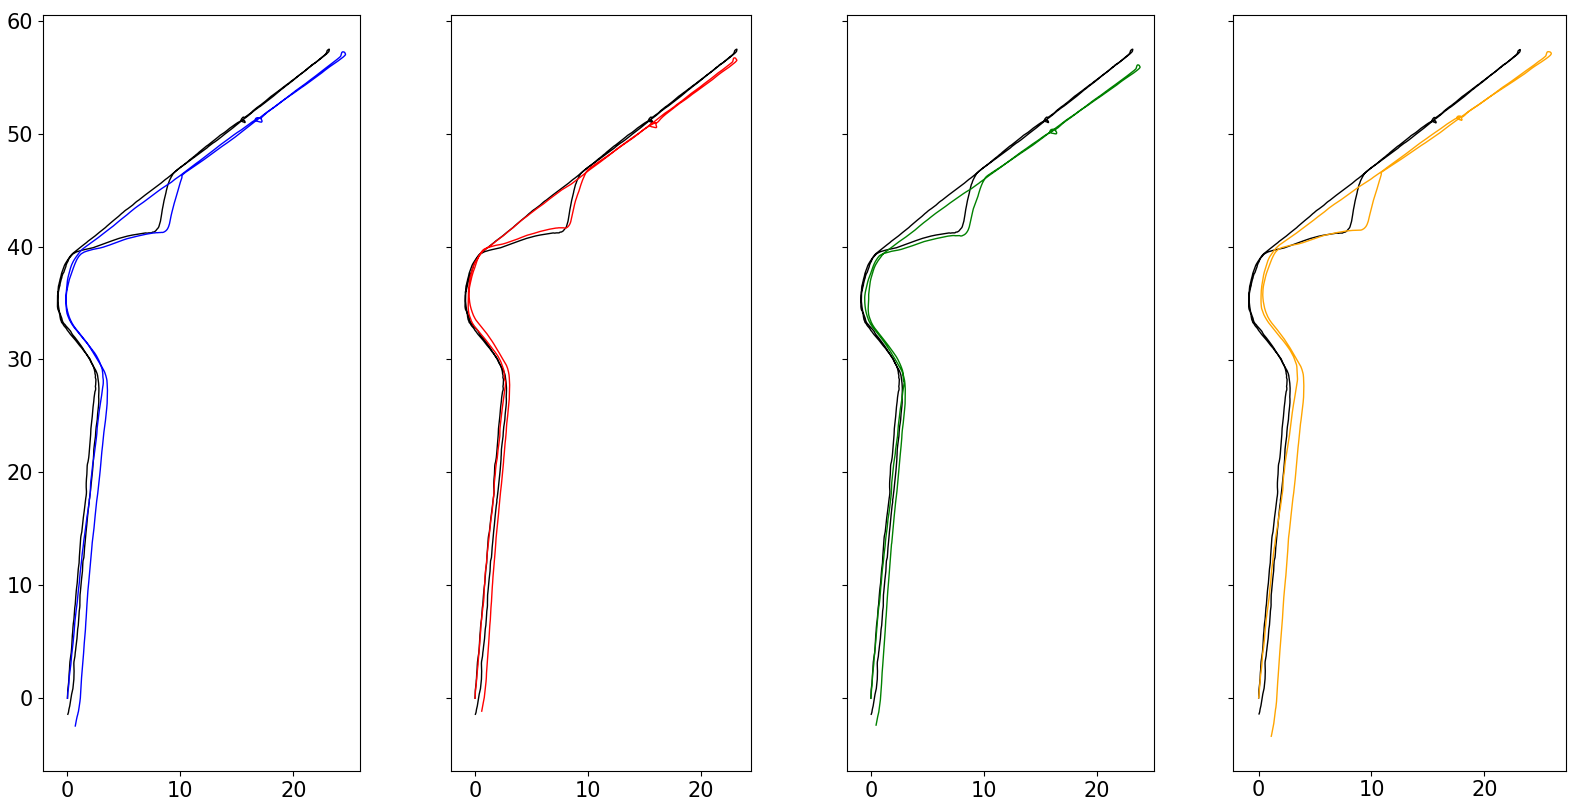
\includegraphics[width=0.85\linewidth]{figures/example_trajectory.png}
%     \caption{Example Trajectory (Run=AF). Black is the ground truth. Blue is with single IMU. Red is with averaged VIMU}
%     \label{fig:posyaw_af}
% \end{figure}

% \begin{figure}[ht!]
%     \centering
%     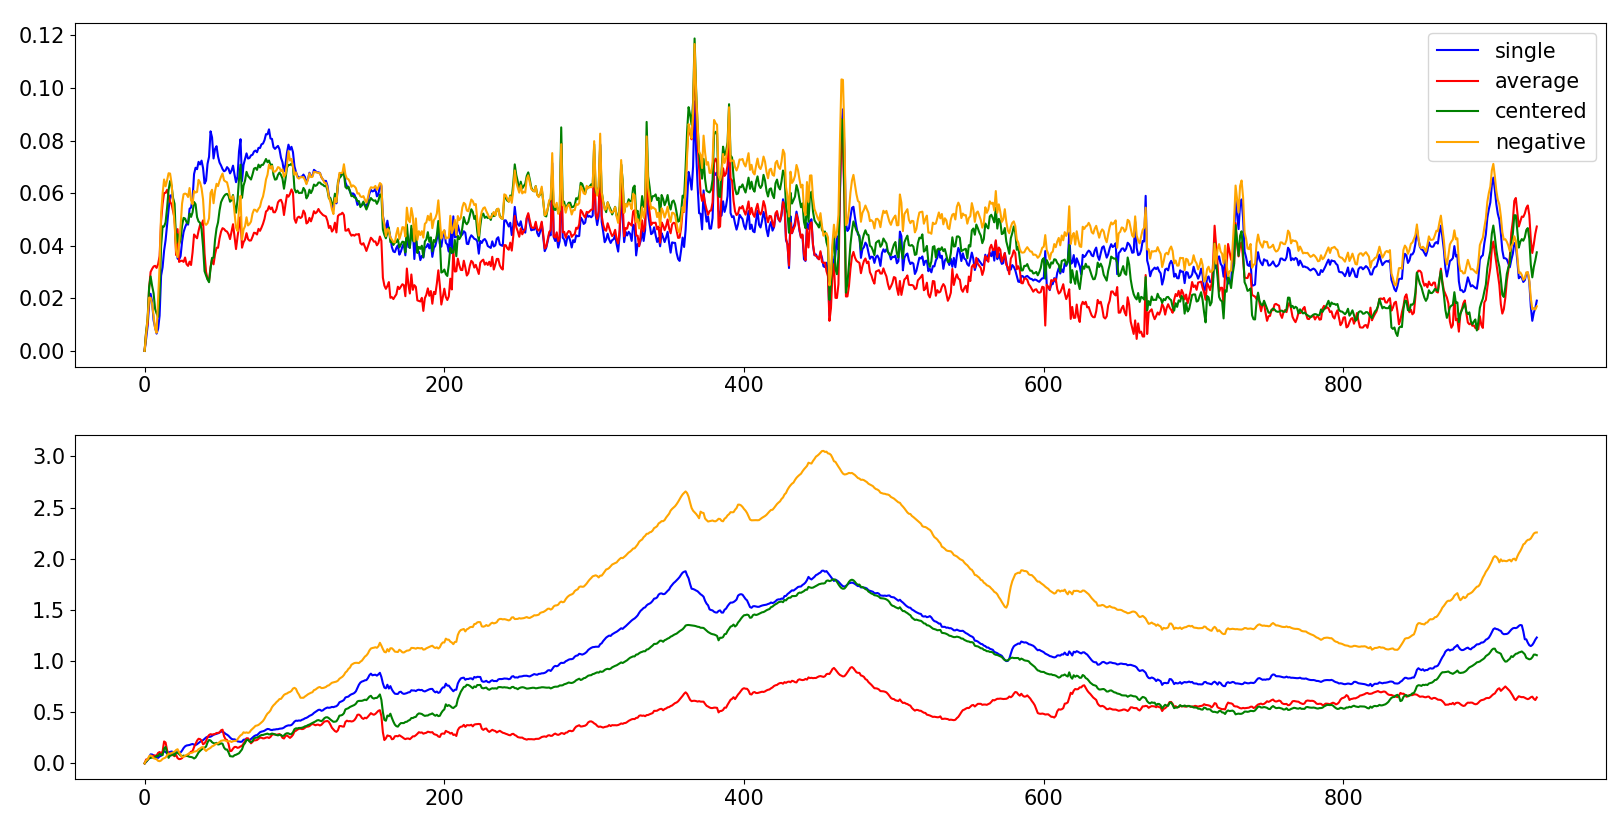
\includegraphics[width=1.0\linewidth]{figures/example_error.png}
%     \caption{Example Error Accumulation over Time (Run=AF). Top is rotational error. Bottom is positional error. \\
%     Single (Blue) Averaged (Red), Centered (Green), Negative (Yellow) }
%     \label{fig:error_af}
% \end{figure}

\begin{figure*}[ht]
    \centering
    \begin{subfigure}[b]{0.45\linewidth}
        \centering
        % \includegraphics[width=7cm]{figures/posyaw_af.png}
        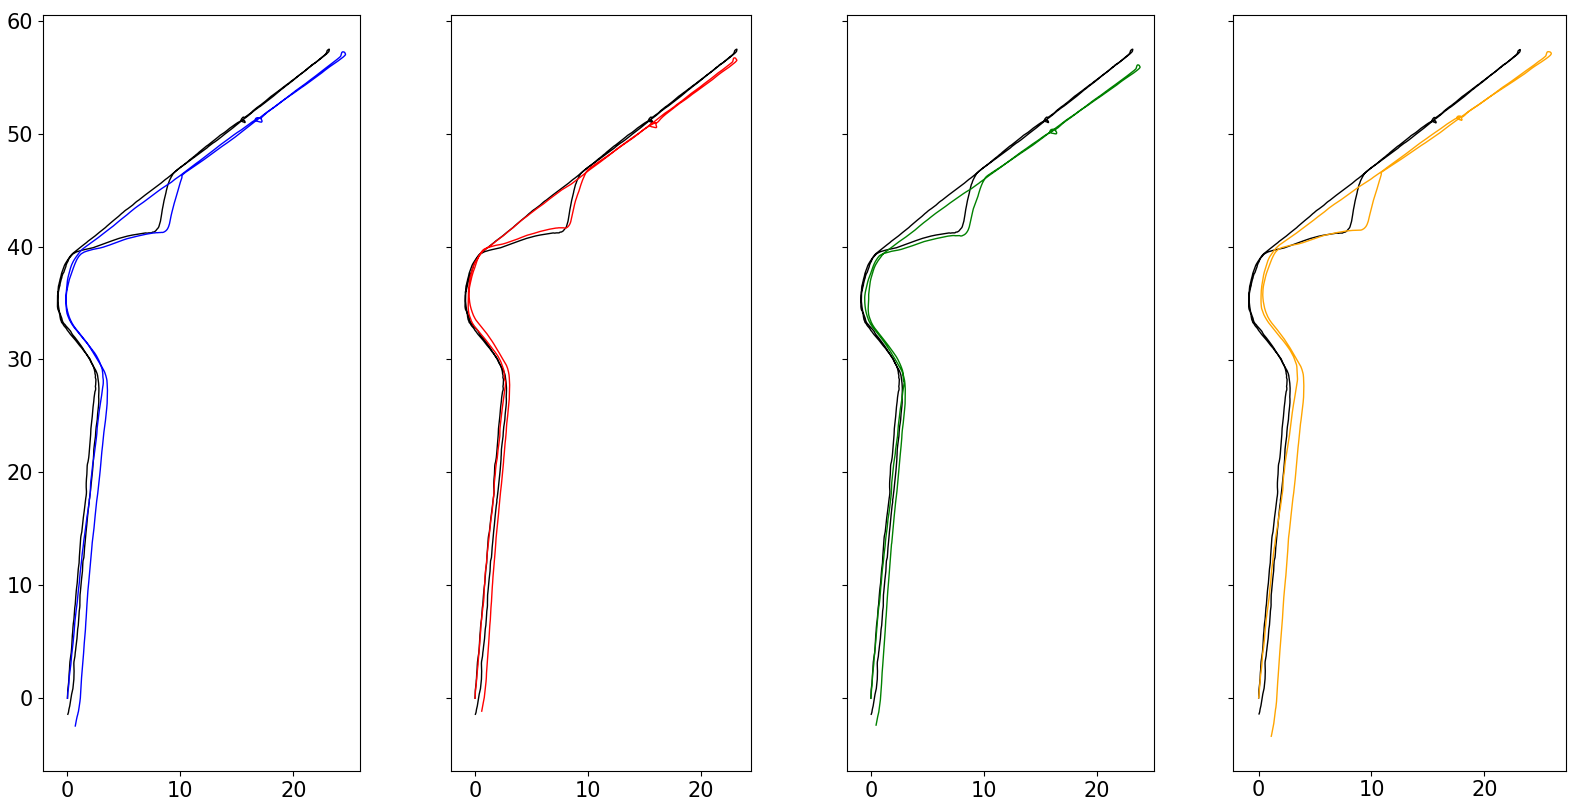
\includegraphics[width=8cm]{figures/example_trajectory.png}
        \caption{Example Trajectories. All trajectories start at (0, 0).}
        \label{fig:posyaw_af}
    \end{subfigure}
    \begin{subfigure}[b]{0.45\linewidth}
        \centering
        % \includegraphics[width=11cm]{figures/error_comp_af_nolabel.png}
        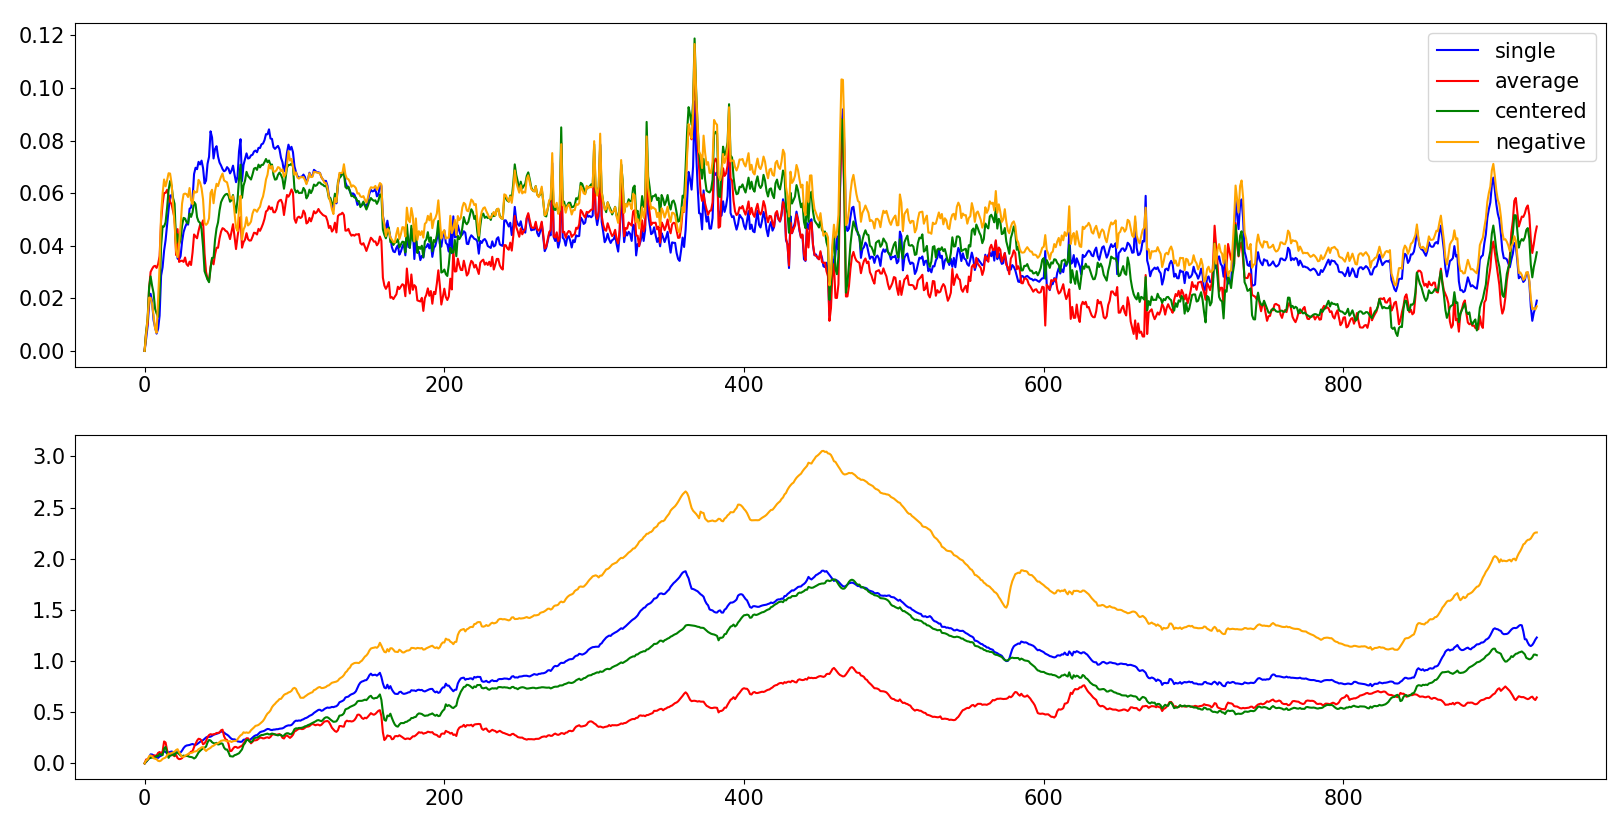
\includegraphics[width=9cm]{figures/example_error.png}
        \caption{Example errors over Time Rot. (Top), Pos. (Bottom).}
        \label{fig:error_af}
    \end{subfigure}
\caption{Example Result for Run AF. Single (Blue) Averaged (Red), Centered (Green), Negative (Yellow)}
\label{fig:real_example}
\end{figure*}

\begin{table}[h!]
\centering
\caption{PennCOSYVIO Results}
\label{tab:vio_result}
\begin{tabular}{cccccc}
\toprule
\textbf{Runs} & \textbf{configurations} & \multicolumn{2}{c}{\textbf{Attitude Err (deg)}} & \multicolumn{2}{c}{\textbf{Position Err (m)}} \\
\cmidrule(lr){3-4} \cmidrule(lr){5-6}
 & & MAE & RMSE & MAE & RMSE \\
\midrule
AF & Single    & 0.0428 & 0.0451 & 1.0031 & 1.0946 \\
AF & Averaged  & \textbf{0.0337} & \textbf{0.0373} & \textbf{0.5051} & \textbf{0.5393} \\
AF & Centered  & 0.0419 & 0.0459 & 0.8258 & 0.9331 \\
AF & Negative  & 0.0505 & 0.0523 & 1.5588 & 1.7128 \\
\midrule
AS & Single    & 0.0400 & 0.0433 & 1.4822 & 1.5485 \\
AS & Averaged  & 0.0421 & 0.0462 & 1.4427 & 1.4902 \\
AS & Centered  & \textbf{0.0324} & \textbf{0.0365} & \textbf{1.3765} & \textbf{1.4387} \\
AS & Negative  & 0.0759 & 0.0821 & 1.7956 & 2.0234 \\
\midrule
BF & Single    & 0.0890 & 0.2983 & 1.1189 & 1.2289 \\
BF & Averaged  & 0.0794 & \textbf{0.2967} & \textbf{0.4917} & \textbf{0.5262} \\
BF & Centered  & \textbf{0.0787} & 0.2967 & 0.7021 & 0.7417 \\
BF & Negative  & 0.1082 & 0.3020 & 3.4679 & 3.6277 \\
\midrule
BS & Single    & 0.0402 & 0.0659 & 1.5926 & 1.7065 \\
BS & Averaged  & 0.0353 & 0.0635 & 2.1734 & 2.2367 \\
BS & Centered  & \textbf{0.0290} & \textbf{0.0592} & \textbf{1.0496} & \textbf{1.1091} \\
BS & Negative  & 0.0490 & 0.0714 & 1.8005 & 1.9496 \\
\bottomrule
\end{tabular}
\end{table}

From the results, we can clearly see that the averaged and centered configuration works better than using a single IMU. This is as expected as averaging can reduce the noise and slow down the bias drift thus result in more accurate tracking of a trajectory. We also see that the negative configuration has larger error over time, this is due to the fact that when the norm of the weight vector goes larger than 1, noises are amplified.

% From the result, different configurations perform similarly. Error reduction from averaging as in simulation is not seen. This is believed to be due to various imperfections from the real-world dataset. For run BF, the large rotation error is due to some incorrect association between estimated trajectory and ground truth.

% 1) Poor calibration. According to the paper of the PennCOSYVIO dataset, the extrinsic calibration is only done between the cameras (for VI sensor only the left camera is calibrated). The IMU positions are assumed from the factory calibration relative to their respective cameras. The chain of transformation introduces large calibration error when averaging the two Tango IMUs with the VI sensor IMU. The VIMU is expected to have less accurate calibration when used with the VI sensor compared to the  built-in IMU.

% 2) No static data. Another issue with the dataset is that there is no static stage at the beginning. The initial static stage is crucial for accurate VIO as it allows estimating the initial biases as well as provides known zero initial velocity. As a result, in OpenVINS we have to rely on dynamic initialization which is less accurate compared to static initialization.

% 3) Vibration and flexing in the fixture. Due to the large separation between all sensors, the physical vibration and deflection in the system can introduce noise and error as well.

% It is expected that the noise improvement from averaging is overwhelmed by the imperfection mentioned above. However, from the result we can still conclude that averaging across multiple IMUs with separation works as expected giving the freedom of placing VIMU frame at preferred location which may not be physically accessible.

\section{Conclusion}

In this paper, we presented that in addition to averaging gyroscopes we can also average multiple accelerometers that are physically separated. We discussed the closed-form solution in determining the weights for placing the VIMU frame at a preferred location while minimizing the measurement noises. Through both simulation and a real dataset experiment, we validated the main concept of VIMU frame placement as well as demonstrated the noise reduction benefit of averaging.

% With real-world dataset, despite the imperfection in the data, we managed to show the averaging technique proposed is a valid approach to take advantage of the redundant IMUs on board. It also reveals the importance of accurate calibration when averaging multiple IMUs. Method of tuning the weights to compensate for the calibration error can be a future work to explore.

\bibliographystyle{plain}
\bibliography{References.bib}

\end{document}
